\section{Initial exploration on CoLA}{
  \label{sec:A-hparam-exploration-cola}
  \subsection{Choosing learning algorithm and learning rate}{
    Because \citet{Tang_2019b} report not tuning their BiLSTM hyperparameters, I verify their choices.
    In particular, the use of the Adam learning algorithm is explored -- a widely used and improved version of the Adadelta algorithm which is used originally.

    For both students, I try a wide range of $\eta$ values with Adam: $5\times10^{-3},\ 1.5\times10^{-3},\ 5\times10^{-4},\ 1.5\times10^{-4},\ 5\times10^{-5},\ 1.5\times10^{-5},\ 5\times10^{-6}$.
    
    \begin{figure}[h!t]
      \centering
      \makebox[\textwidth][c]{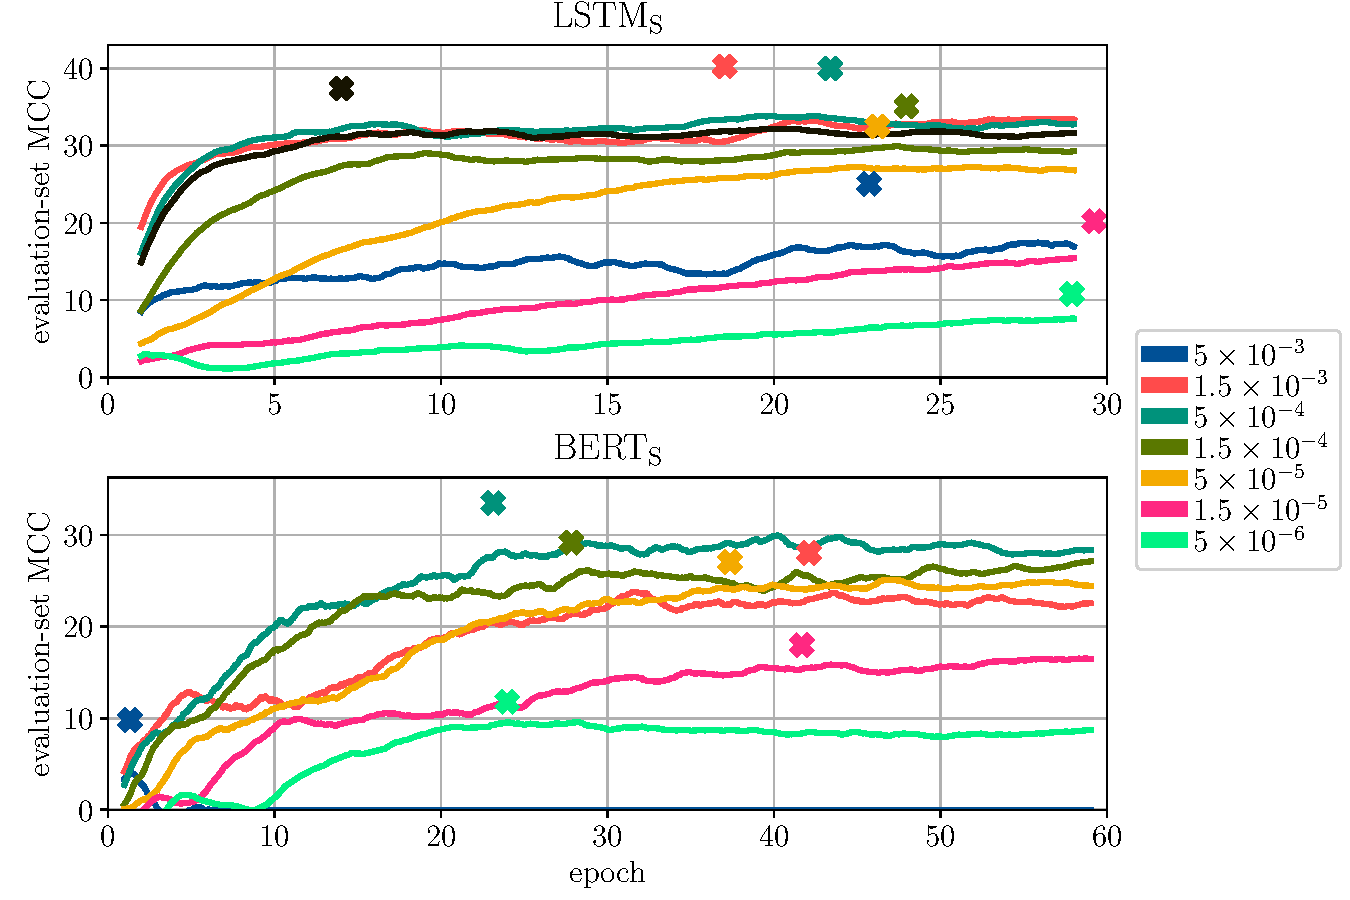
\includegraphics[width=14.8cm]{../experiments/analysis/img/exploration-lr}}
      \caption{Comparing various $\eta$ values on CoLA. Crosses mark the maximum scores. \sliding~In particular, notice that the best-score points (crosses) are well above the smoothed lines -- this is because the (unsmoothed) evaluation score varies a lot, as illustrated in the upper plot for \LSTMS~with $\eta=5\times10^{-3}.$}
      \label{fig:exploration-lr}
    \end{figure}

    \autoref{fig:exploration-lr} shows that for all students the ideal $\eta$ is around $5\times10^{-4}$. Much larger and much smaller values leading to poor learning, in particular the largest $\eta=5\times10^{-3}$ ``kills'' the learning of \BERTS~entirely due to gradient explosion.
    As expected, \BERTS~initialised from scratch performs worse than when initialised from the wordpiece embeddings of \BERTT. However, the differences are not large.

    As discussed previously, \BERTS~converges much slower than \LSTMS, hence the 30-epoch and 60-epoch training budgets for \LSTMS~and \BERTS, respectively. Additionally, it is apparent that \LSTMS~performs significantly better than \BERTS~even though the sizes of the models are comparable.

    In the case of \LSTMS, the Adadelta algorithm is outperformed by Adam. From now onwards, I use Adam with both students, in all cases with $\eta=5\times10^{-4}$.
  }

  \subsection{Choosing learning rate scheduling and batch size}{
    \citet{Tang_2019a} use no learning rate scheduling, but they report small batch sizes ($B=50$) to work better than the usual, larger batches. Hence, for \LSTMS~I first verify their claims and subsequently move on to $\eta$ scheduling. For \BERTS, inspired by \citet{Sanh_2019} who take advantage of scheduling (both in terms of warmup and decay), I explore $\eta$ scheduling first (as a continuation from exploring $\eta$ values), and then look at various $B$ values.

    \begin{figure}[h!t]
      \centering
      \makebox[\textwidth][c]{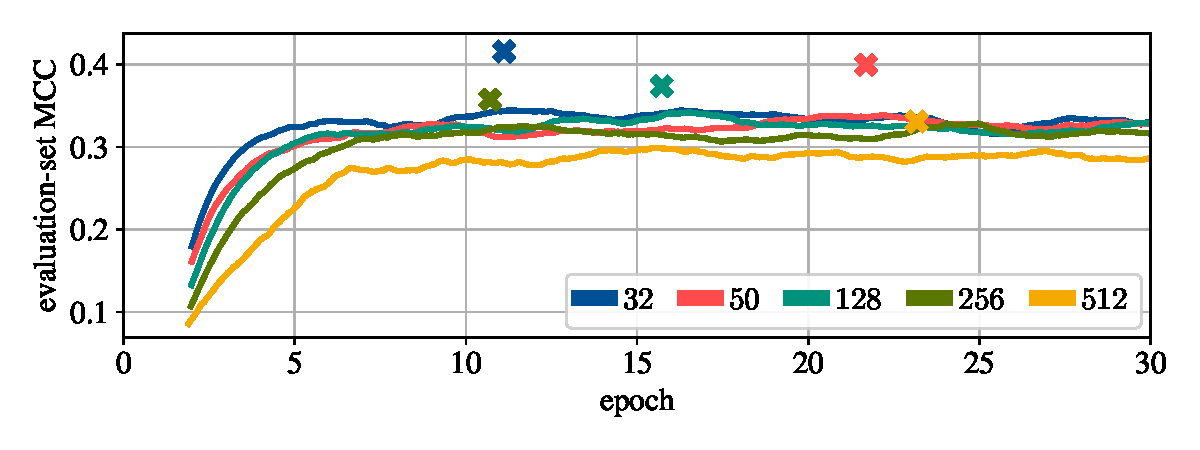
\includegraphics[width=14cm]{../experiments/analysis/img/exploration-B-lstm}}
      \caption{Comparing various batch sizes for \LSTMS~on CoLA. Crosses mark the maximum scores. \sliding}
      \label{fig:exploration-B-lstm}
    \end{figure}

    As \autoref{fig:exploration-B-lstm} shows, \LSTMS~clearly does prefer small batch sizes. However, training with tiny minibatches takes very long -- compare \mytilde25min for $B=512$ with \mytilde7h for $B=32$. Hence, I restrain from trying even smaller batch sizes and use $B=32$ for \LSTMS~in all further experiments.

    \begin{figure}[h!t]
      \centering
      \makebox[\textwidth][c]{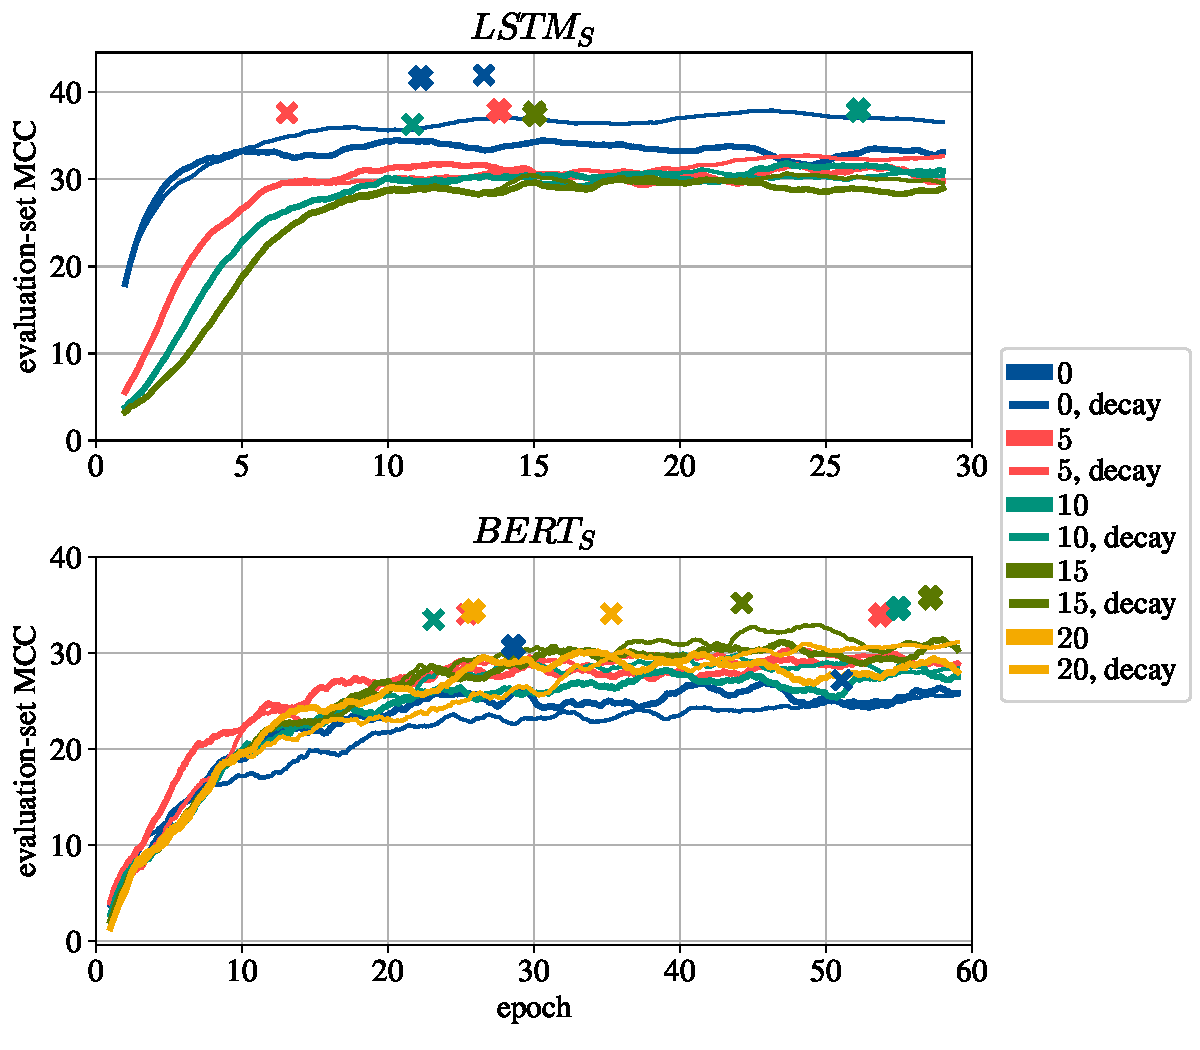
\includegraphics[width=13.5cm]{../experiments/analysis/img/exploration-schedule}}
      \caption{Comparing warmup durations $E_w$ on CoLA, with the optional learning rate decay to 0 over the remaining training epochs. Crosses mark the maximum scores. \sliding}
      \label{fig:exploration-schedule}
    \end{figure}

    \autoref{fig:exploration-schedule} shows the results of exploring various warmup durations for both students. Note that for \LSTMS, whose training budget is only 30 epochs, I did not try the long warmup duration of 20 epochs, only up to 15 epochs.

    In the case of \LSTMS, \autoref{fig:exploration-schedule} shows that the longer the warmup duration, the slower the model converges. This is understandable because during warmup, learning happens less aggressively -- and hence more slowly -- due to the smaller learning rate. More importantly, the graph shows that $\eta$ decay does not significantly affect training, but it can help to prevent the model from overfitting the training data. This is most visible for $E_w=0$ where \LSTMS's performance starts to slowly decrease after 20 epochs in the absence of $\eta$ decay. All in all, using the full $\eta$ from the beginning of training is the best option, and $\eta$ decay can only improve things. $E_w=0$ with decay is used for \LSTMS~in all further experiments.

    In the case of \BERTS, the only clear result visible from \autoref{fig:exploration-schedule} is that \BERTS~performs poorly without $\eta$ warmup. For non-zero warmup durations, there are no significant differences in the best-performance points (marked by crosses) or in the convergence speed. In all further experiments with \BERTS, I use $E_w=15$ and $\eta$ decay -- the configuration which shows the highest stable performance level in \autoref{fig:exploration-schedule} in later epochs (beyond epoch 35).

    \begin{figure}[h!t]
      \centering
      \makebox[\textwidth][c]{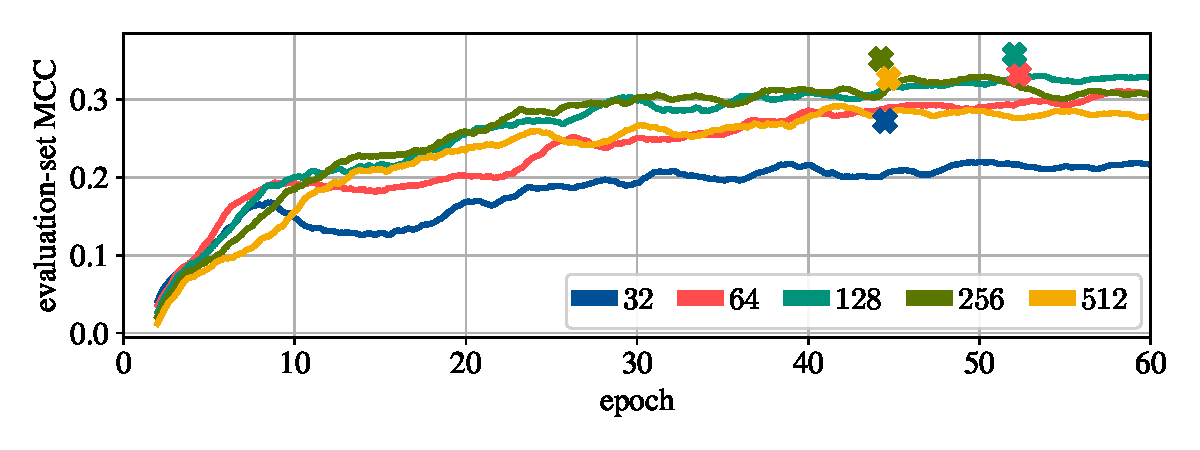
\includegraphics[width=14cm]{../experiments/analysis/img/exploration-B-bert}}
      \caption{Comparing various batch sizes for \BERTS~on CoLA. Crosses mark the maximum scores. \sliding}
      \label{fig:exploration-B-bert}
    \end{figure}

    The batch size exploration in \autoref{fig:exploration-B-bert} shows that \BERTS~performs best with mid-sized batches of 128-256 examples. Too large batch size ($B=512$) as well as very small batches of 32-64 make \BERTS~underperform (with tiny batches of 32 being particularly detrimental).
    In all further experiments, $B=128$ is used with \BERTS.
  }
}

\section{Optimising students for each downstream task}{
  In this section, I provide details of explore different ways of initialising student models with language knowledge, and the effect of model size, separately for each downstream task.

  \subsection{Choosing embedding type and mode}{
    \label{sec:A-exploration-embed}
    \begin{figure}[h!t]
      \centering
      \makebox[\textwidth][c]{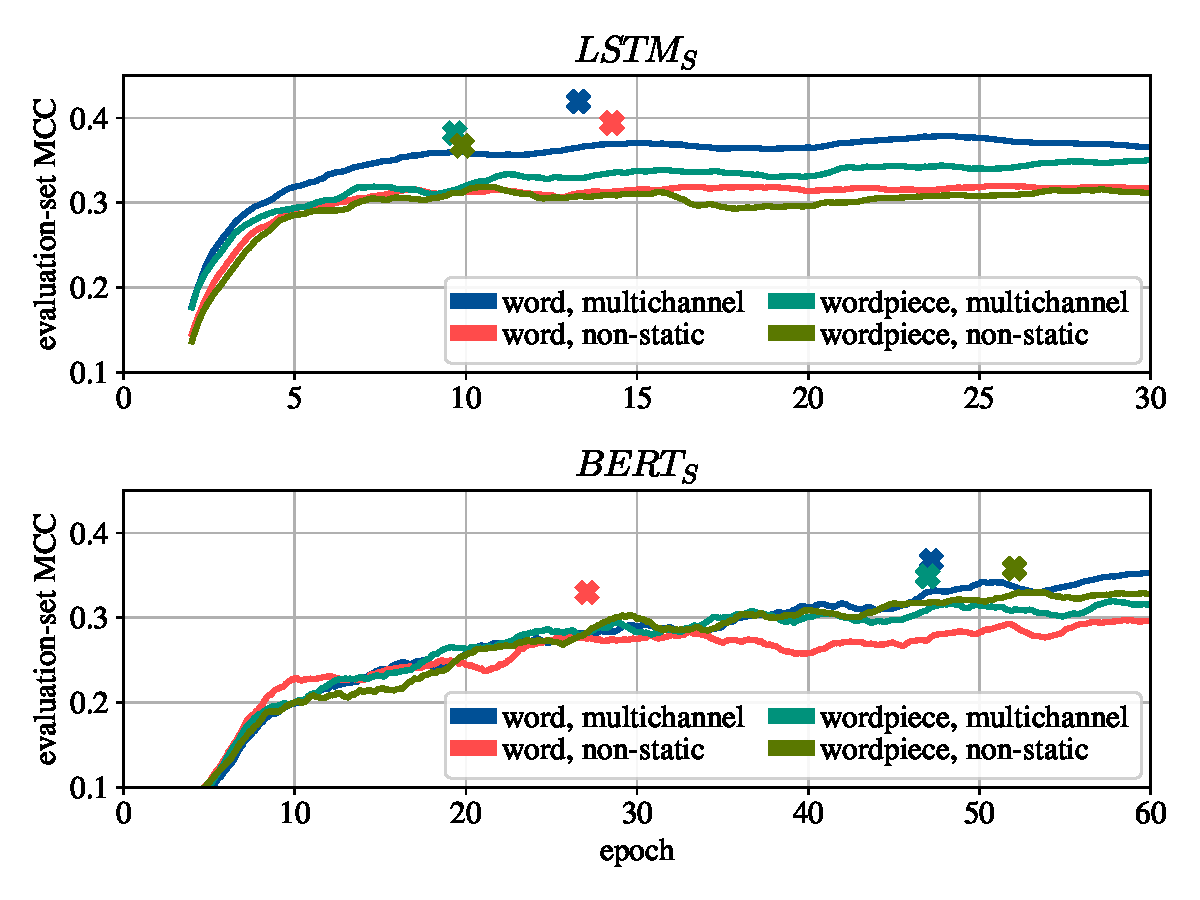
\includegraphics[width=14cm]{../experiments/analysis/img/exploration-embed-cola}}
      \caption{Comparing embedding types and modes on CoLA. Crosses mark the maximum scores. \sliding}
      \label{fig:exploration-embed-cola}
    \end{figure}

    \autoref{fig:exploration-embed-cola} shows how different type and mode combinations affect knowledge distillation on CoLA. With \LSTMS, the multichannel mode is preferred to non-static and word2vec embeddings are preferred to wordpieces; hence, I use the multichannel mode with word2vec in further experiments (same as \citet{Tang_2019b}). For \BERTS, the differences are smaller, yet it is clear that word-level embeddings benefit from using the frozen and unfrozen versions provided by the multichannel mode. In further experiments, the multichannel mode combined with word-level word2vec embeddings is used.

    For SST-2, I only compare the best word-level and the best wordpiece-level combination for each model as observed from \autoref{fig:exploration-embed-cola}. The results are shown in \autoref{fig:exploration-embed-sst-2}. Notice the scale of the y axis: In particular, the students perform roughly the same (unlike on CoLA) and any relative differences observed in \autoref{fig:exploration-embed-sst-2} are much smaller than the differences observed on CoLA in \autoref{fig:exploration-embed-cola}. Hence, I refrain from making conclusions about which embedding type and mode works better; I merely choose to use the word-level embeddings with the multichannel mode in all further experiments on SST-2 (my decision is based on the best evaluation scores marked by crosses in \autoref{fig:exploration-embed-sst-2}).

    \begin{figure}[h!t]
      \centering
      \makebox[\textwidth][c]{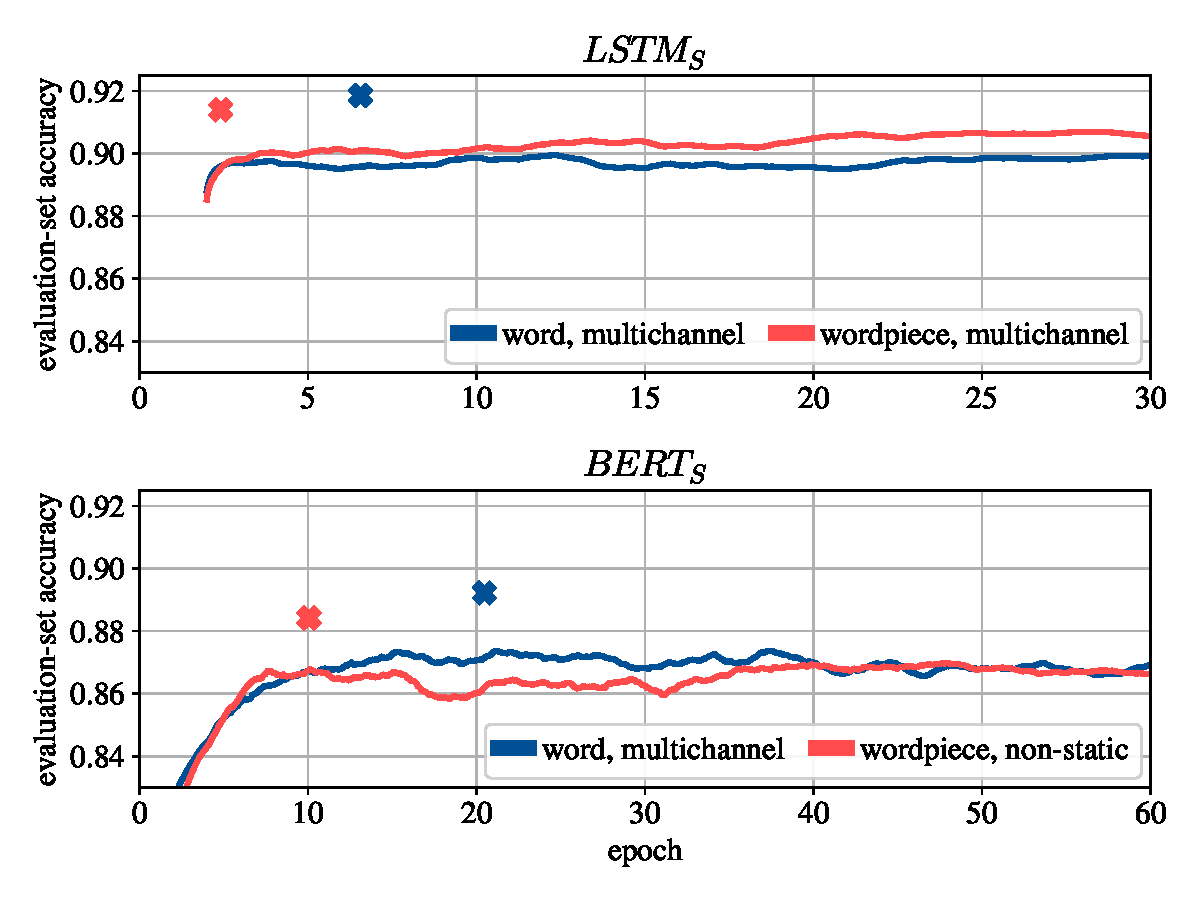
\includegraphics[width=14cm]{../experiments/analysis/img/exploration-embed-sst-2}}
      \caption{Comparing embedding types and modes on SST-2. Crosses mark the maximum scores. \sliding}
      \label{fig:exploration-embed-sst-2}
    \end{figure}

    Results on Sara are shown in \autoref{fig:exploration-embed-sara}. Here again, the relative differences in performance are small, but using wordpieces helps both students converge faster and reach slightly better performance levels. This can be a result of the word2vec vocabulary not capturing well the conversational language in Sara examples, for instance the utterance ``yesyesyes'' would be treated simply as one out-of-vocabulary word, whereas wordpieces have the potential to encode it as the word ``yes'' repeated 3x. In all further experiments on Sara I use the wordpiece embeddings, using the multichannel mode in \LSTMS~and the non-static mode in \BERTS.

    \begin{figure}[h!t]
      \centering
      \makebox[\textwidth][c]{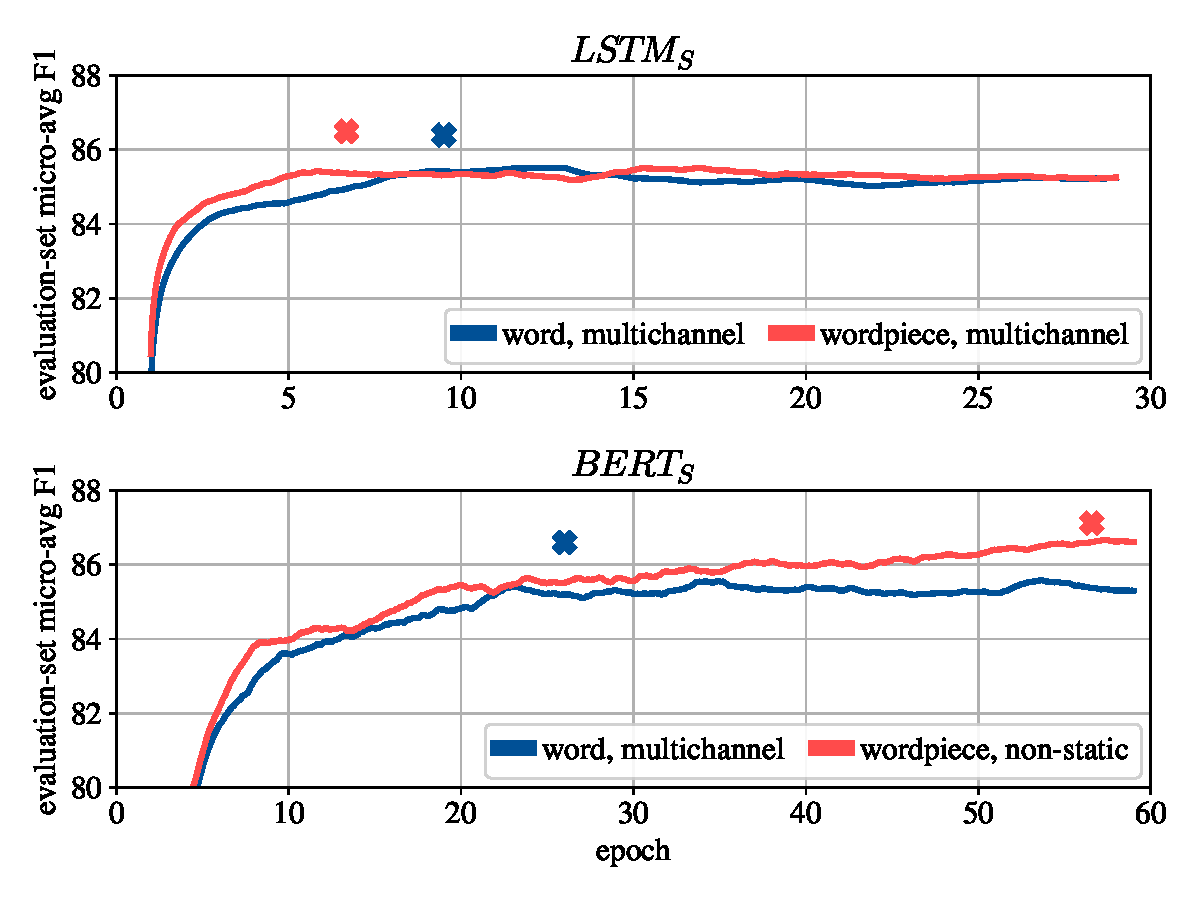
\includegraphics[width=14cm]{../experiments/analysis/img/exploration-embed-sara}}
      \caption{Comparing embedding types and modes on Sara. Crosses mark the maximum scores. \sliding}
      \label{fig:exploration-embed-sara}
    \end{figure}

    All in all, the multichannel mode seems to be generally superior to the non-static mode which lacks the frozen version of embeddings. Initialisation from the word-level word2vec embeddings also works better than wordpieces where examples tend to contain legitimate English (CoLA and SST-2). As for the performance gap between \LSTMS~and \BERTS, I conclude that it cannot be explained by differences in embedding type/mode, and is most likely a consequence of different student architectures.

    While wordpiece embeddings have the advantage of being fine-tuned on the particular downstream task (as part of teacher fine-tuning), word2vec contains more general knowledge stored at the word level.
    Importantly, the wordpiece vocabulary contains the most frequent words in their entirety; only the less frequent ones are split into pieces.
    Thus, for frequent words, their word2vec and wordpiece embeddings will differ only in the way they are trained.
    Naturally, since the wordpiece vocabulary has only 30,522 tokens while word2vec has 3,000,000, there are many words covered by word2vec for which the wordpiece embeddings have to be assembled from multiple pieces. On these words -- frequent enough to be in the word2vec vocabulary, but not the most frequent ones -- word2vec could have an advantage.
    Once we move beyond the words covered by word2vec to rare tokens like ``yesyesyes'', wordpieces become the preferred approach.
    Clearly, no one approach is generally the best, and the decision should ideally be made individually for each downstream task.
  }

  \subsection{Choosing student size}{
    \label{sec:A-student-size}
    As the last parameter, I explore the size of each student. In particular, I try to reduce the performance gap on CoLA between \BERTT~and both students by making the students larger. On SST-2 and Sara, the 2.4-million-parameter students already achieve scores very close to those of the teacher, and I refrain from exploring larger students -- instead, I explore smaller student sizes.

    There are two main ways of increasing the student size: By increasing the model ``width'' and the ``depth''. By width, I mean the dimensionality of the model's layers and internal representations. Depth means adding more layers. While larger width allows the models to extract and maintain richer token representations, adding layers adds more steps to the models' processing pipelines, allowing for more abstract and task-specific representations to be extracted in the end.

    In \BERTS, I manipulate width by increasing by a set factor $W$ the hidden dimensionality $d_h$, the intermediate dimensionality $d_I$, and the number of self-attentional heads $A$. Depth is manipulated by changing the number of encoder layers $L$ by the factor $D$.
    In \LSTMS, I change model width by scaling by $W$ the LSTM layer width $d_{LSTM}$ and the fully-connected layer width $d_{FC}$, which are originally set to 300 and 400, respectively. Depth is changed by increasing the number of LSTM layers (originally just one) by the factor $D$.
    The concrete dimensions of up- and down-scaled students are shown in \autoref{tab:sizes-bert} (\BERTS) and in \autoref{tab:sizes-lstm} (\LSTMS).

    \begin{table}[h!t]
    \centering
    \begin{tabular}{c|ccc}
    \hline
    $W$ & $d_h$           & $d_I$               & $A$ \\ 
    \hline
    1/16& 13              & 47                  & 1   \\
    1/8 & 26              & 94                  & 1   \\
    1/4 & 51              & 188                 & 1   \\
    1/3 & 68              & 250                 & 1   \\
    1/2 & 102             & 375                 & 2   \\
    1   & 204             & 750                 & 3   \\
    2   & 408             & 1500                & 6   \\
    3   & 612             & 2250                & 9   \\
    4   & 816             & 3000                & 12  \\
    % 5   & 1020            & 3750                & 15  \\
    \hline
    \end{tabular}
    \quad \quad \quad \quad
    \begin{tabular}{c|c}
    \hline
    $D$ & $L$ \\
    \hline
    1/4 & 1   \\
    1/3 & 2   \\
    1/2 & 3   \\
    1   & 5   \\
    2   & 10  \\
    3   & 15  \\
    \hline
    \end{tabular}
    \caption{\BERTS~dimensions for different width scalings (left) and depth scalings (right). The default size with 2.4 million parameters corresponds to $W=1$, $D=1$.}
    \label{tab:sizes-bert}
    \end{table}

    \begin{table}[h!t]
    \centering
    \begin{tabular}{c|cc}
    \hline
    $W$ & $d_{LSTM}$  & $d_{FC}$\\ 
    \hline
    1/32& 9           & 13 \\
    1/16& 19          & 25 \\
    1/8 & 37          & 50 \\
    1/4 & 75          & 100 \\
    1/2 & 150         & 200 \\
    1   & 300         & 400 \\
    2   & 600         & 800 \\
    3   & 900         & 1200 \\
    4   & 1200        & 1600 \\
    5   & 1500        & 2000 \\
    \hline
    \end{tabular}
    \quad \quad \quad \quad
    \begin{tabular}{c|c}
    \hline
    $D$ & $L$ \\
    \hline
    1   & 1  \\
    2   & 2  \\
    3   & 3  \\
    4   & 4  \\
    5   & 5  \\
    \hline
    \end{tabular}
    \caption{\LSTMS~dimensions for different width scalings (left) and depth scalings (right). The default size with 2.4 million parameters corresponds to $W=1$, $D=1$.}
    \label{tab:sizes-lstm}
    \end{table}

    \subsubsection{CoLA}{
      With the teacher's evaluation-set MCC of 59.9 being much higher than the student performance observed so far (around 40), I up-scale both students, aiming for 90\% of the teacher performance while keeping the student size smaller than the 340-million-parameter teacher.

      As observed in preliminary experiments with large \BERTS~versions, their learning suffers from gradient explosion due to the learning rate being too large for the models. For an example, see \autoref{fig:exploding-grads} where the gradient explosion happens around epoch 7 and the model score (MCC) then falls to 0 and stays there.

      \begin{figure}[h!t]
        \centering
        \makebox[\textwidth][c]{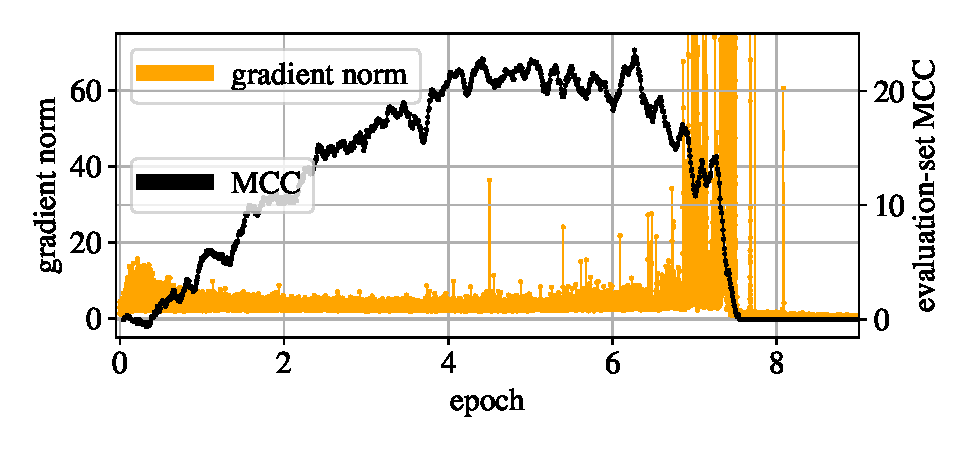
\includegraphics[width=12cm]{../experiments/analysis/img/exploding-grads}}
        \caption{Gradient explosion in \BERTS~with $W=2$ and $D=2$. The MCC values have been smoothed with a 0.1-epoch-wide sliding average window.}
        \label{fig:exploding-grads}
      \end{figure}

      Without further extensive exploration of optimal learning rate values for each \BERTS~size\footnote{This would be extremely time-consuming because the larger versions take over 3 days to train.}, I choose better learning rate values manually.
      Because of the use of $\eta$ warmup, I can monitor the learning progress for varying $\eta$ values in the early training epochs, as shown in \autoref{fig:exploding-grads-choosing-lr}. I approximately identify the point in training beyond which the learning slows down (and later degrades altogether) due to large gradients. This way, I approximately identify the largest learning rate that still leads to learning, not to gradient explosion. In the concrete example in \autoref{fig:exploding-grads-choosing-lr}, I choose the point in training after 2.5 epochs, where the learning rate is approximately $\eta=8\times10^{-5}$, and use this value with the concrete model size.
      
      \begin{figure}[h!t]
        \centering
        \makebox[\textwidth][c]{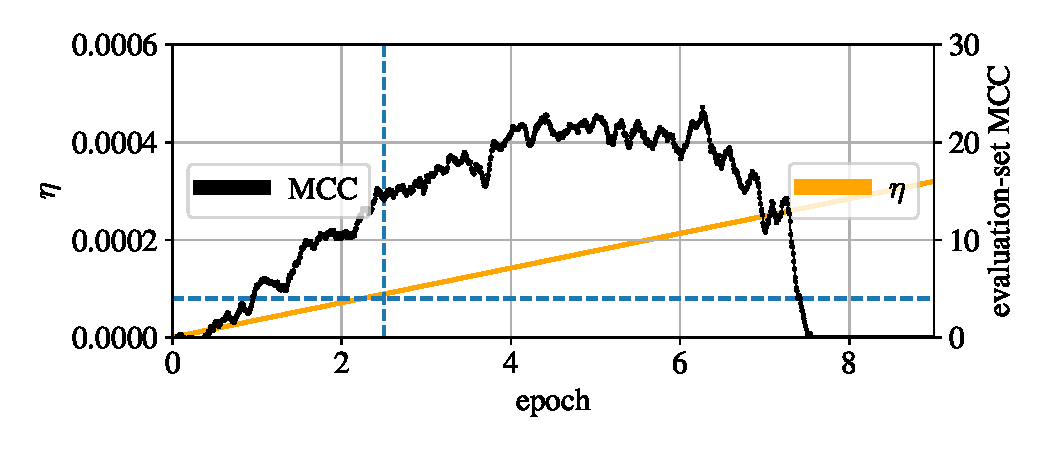
\includegraphics[width=12cm]{../experiments/analysis/img/exploding-grads-choosing-lr}}
        \caption{Learning progress (MCC over time) vs $\eta$ for \BERTS~with $W=2$ and $D=2$ -- the model experiencing gradient explosion in \autoref{fig:exploding-grads}. The dashed lines show the position I identify as the approximate latest point of training before the learning starts to slow down, and the learning rate at that position.
        The MCC values have been smoothed with a 0.1-epoch-wide sliding average window.}
        \label{fig:exploding-grads-choosing-lr}
      \end{figure}

      With the new learning rates manually estimated individually for each student size, none of the larger versions of \BERTS~experiences gradient explosion. The LSTM students all use the same learning rate as this does not lead to any issues. \autoref{fig:size-cola} presents the results. While some larger students outperform the original, 2.4-million-parameter ones, the trends are not consistent. For \LSTMS~in particular, there is no clear correlation between student width or depth and the performance. For \BERTS, which starts as a relatively deep model with 5 layers, making it wider rather than deeper is helpful. For \LSTMS~which originally has only 1 hidden LSTM layer, increasing both the width and the depth can lead to better-performing models. Overall, both student architectures reach the best evaluation score of \mytilde45, far below the teacher performance level of 59.9. 

      \begin{figure}
        \centering
        \begin{subfigure}{.5\textwidth}
          \centering
          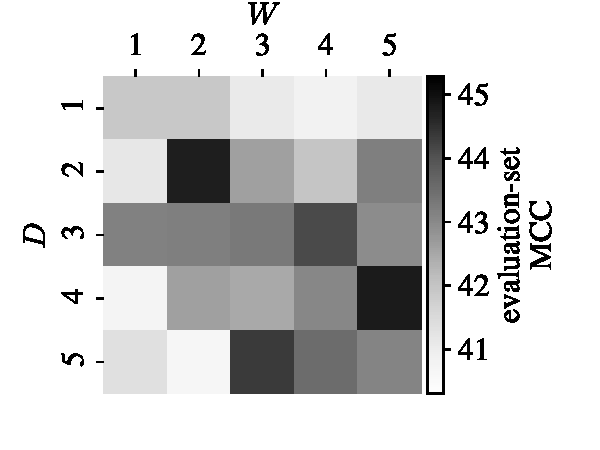
\includegraphics[width=7cm]{../experiments/analysis/img/size-cola-lstm-map}
          \caption{Different sizes of \LSTMS.}
          \label{fig:size-cola-lstm}
        \end{subfigure}%
        \begin{subfigure}{.5\textwidth}
          \centering
          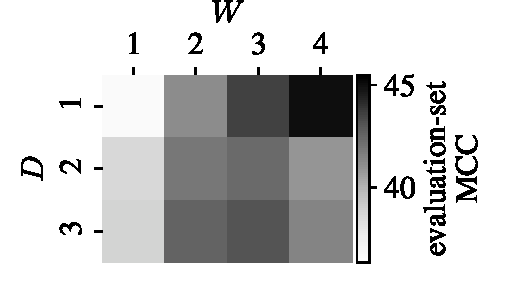
\includegraphics[width=6.5cm]{../experiments/analysis/img/size-cola-bert-map}
          \caption{Different sizes of \BERTS.}
          \label{fig:size-cola-bert}
        \end{subfigure}
        \caption{Best evaluation-set performance for the different student sizes on CoLA.}
        \label{fig:size-cola}
      \end{figure}
      
      I refrain from exploring students even larger as the biggest students are already approching the teacher size: \LSTMS~with $W=5$, $D=5$ has \mytilde247 million parameters and takes over 60h to train, and \BERTS~with $W=4$, $D=3$ has \mytilde114 million parameters and takes over 6 days to train.
      As the best-performing students, I establish \BERTS~with $W=4$, $D=1$, and \LSTMS~with $W=2$, $D=2$.
    }

    \subsubsection{SST-2}{
      As previously observed, on SST-2, even the default 2.4-million-parameter students perform on par with the teacher. With no reason to try larger student sizes, I limit myself to exploring smaller student architectures, with the aim of keeping student accuracy above 90\% of the teacher's score. With \BERTT~achieving 91.5\% accuracy, the 90\% lower bound is at \mytilde82\% accuracy.

      \autoref{fig:size-sst-2} shows that accuracy stays high even for very small students. 
      The smallest tried LSTM student ($W=1/64$, 24,360 non-embedding parameters, \mytilde14,000x smaller than \BERTT) still achieves 89.1\% accuracy (\mytilde97\% of the teacher's performance).
      The smallest tried BERT student ($W=1/16$, $D=1/4$, 2272 non-embedding parameters, \mytilde150,000x smaller than \BERTT) achieves 83.5\% accuracy (\mytilde91\% of \BERTT's performance).
      What these results mean is that the SST-2 task is relatively easy. 
      For good accuracy levels, a very minimalistic classifier is sufficient on top of the pre-trained embeddings -- the representations obtained simply by encoding each word using word2vec already contain most of the knowledge needed to make good sentiment predictions.

      \begin{figure}
      \makebox[\linewidth][c]{%
        \centering
        \begin{subfigure}{.61\textwidth}
          \centering
          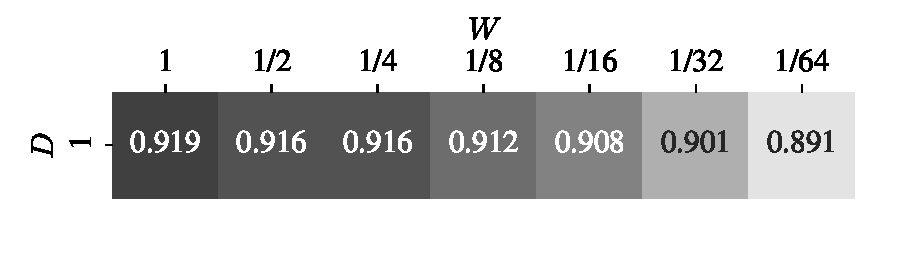
\includegraphics[width=9cm]{../experiments/analysis/img/size-sst-2-lstm-map}
          \caption{Different sizes of \LSTMS.}
          \label{fig:size-sst-2-lstm}
        \end{subfigure}%
        \begin{subfigure}{.5\textwidth}
          \centering
          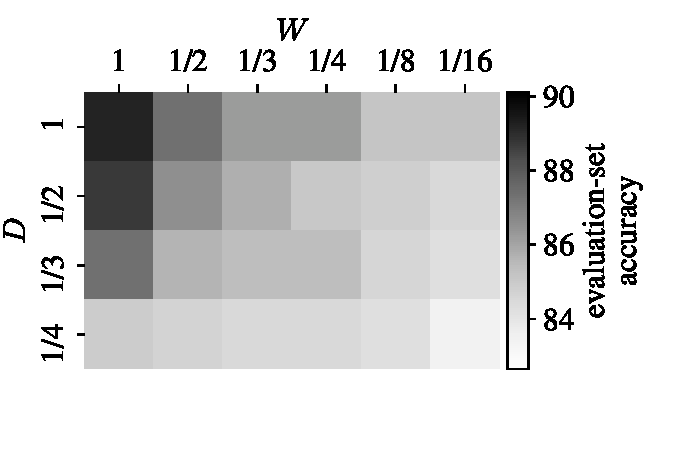
\includegraphics[width=7.5cm]{../experiments/analysis/img/size-sst-2-bert-map}
          \caption{Different sizes of \BERTS.}
          \label{fig:size-sst-2-bert}
        \end{subfigure}
      }
      \caption{Best evaluation-set performance for the different student sizes on SST-2.}
      \label{fig:size-sst-2}
      \end{figure}
      Another insight from \autoref{fig:size-sst-2-bert} is that making \BERTS~shallower affects the performance much less than making it slimmer. In other words, the 2.4-million-parameter \BERTS~may be unnecessarily deep for the task, but it is not unnecessarily wide.
    }

    \subsubsection{Sara}{
      Similar to SST-2, Sara is an easy task. With \BERTT~achieving $F_{1 micro}=87.5$, the 2.4-million-parameter \BERTS~and \LSTMS~already achieve 87.1 and 86.5, respectively.
      I further down-scale the students, see \autoref{fig:size-sara}. Similar to the results on SST-2, both students can be made much smaller while achieving over 90\% of \BERTT's performance.
      The second smallest tried \LSTMS~($W=1/4$) is 262x smaller than the teacher while retaining almost 95\% of its performance.
      The \BERTS~with $W=1/2$ and $D=1/4$, being 2500x smaller than \BERTT, retains \mytilde93\% of its performance.

      Also similarly to SST-2, making \BERTS~shallower has much weaker effect on the performance than making it thinner. In other words, the Sara task does not require very deep models, and keeping the representation dimensionality above certain level (in this case around 128 or above, corresponding to $W\geq1/2$) is more important.
      \begin{figure}
      \makebox[\linewidth][c]{%
        \centering
        \begin{subfigure}{.61\textwidth}
          \centering
          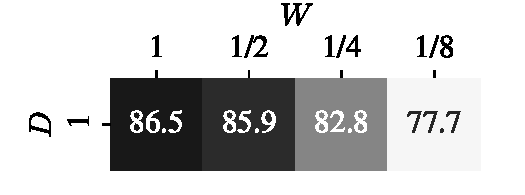
\includegraphics[width=5.4cm]{../experiments/analysis/img/size-sara-lstm-map}
          \caption{Different sizes of \LSTMS.}
          \label{fig:size-sara-lstm}
        \end{subfigure}%
        \begin{subfigure}{.5\textwidth}
          \centering
          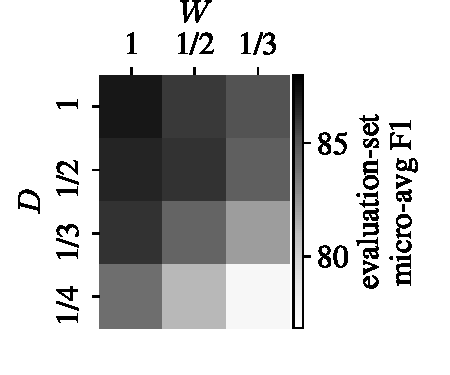
\includegraphics[width=5cm]{../experiments/analysis/img/size-sara-bert-map}
          \caption{Different sizes of \BERTS.}
          \label{fig:size-sara-bert}
        \end{subfigure}
      }
      \caption{Best evaluation-set performance for the different student sizes on Sara.}
      \label{fig:size-sara}
      \end{figure}
    }
  }
}
